\documentclass[11pt]{amsart}
\usepackage[centering]{geometry}           % See geometry.pdf to learn the layout options. There are lots.
\geometry{a4paper} % ... or a4paper or a5paper  or ... letterpaper
%\geometry{landscape}                % Activate for for rotated page geometry
%\usepackage[parfill]{parskip}    % Activate to begin paragraphs with an empty line rather than an
%indent
\usepackage{graphicx}
\usepackage{amssymb}
\usepackage{epstopdf}
\usepackage{amsmath}
\DeclareGraphicsRule{.tif}{png}{.png}{`convert #1 `dirname #1`/`basename #1 .tif`.png}






\title{Tidal Asteroseismology}
\author{Andrew Bunting}
%\date{}                                           % Activate to display a given date or no date
%
\begin{document}

\maketitle

\section{Introduction}

Stars are ubiquitous in almost all areas of astrophysics, and it is becoming increasingly apparent that planets are a common occurrence as well.  My project revolves around the interaction between a subset of these two very common objects, and will enable us to test our understanding of what is going on inside the stars, and also could help in the hunt for planets.

Over the course of the introduction I will set out the background to the project, including setting it in a (brief) history of the relevant areas, covering: Asteroseismology, Stellar Oscillations, Stellar Structure, Exoplanets and Tidal Asteroseismology.  In the sections following that, I will cover in some more detail the Henyey method, the implementation of the method for this particular set of equations, and the outputs generated by the code; I will end with a conclusion of what has been achieved, and a plan for future work to further these achievements.







\subsection{Asteroseismology}

Variable stars have been observed for over $3000$ years \cite{Jetsu2015}, although only in the last few centuries has the number of observed variable stars really grown \cite{Hoffleit1997}.  That stars are not constant was a major change from the classical view of the celestial sphere, and adds many layers to the complexity of stars, but also introduces new ways for us to learn about them.  Asteroseismology is the study of stellar oscillations, and is a rapidly growing field, as the quality of observations of stellar surfaces continues to improve.

Asteroseismology, understandably, first came about in studying the oscillations of our very own star -- potentially the first such vibrations were observed by Plaskett in 1916 \cite{Plaskett1916}, although the  observed variation in solar rotation was thought to be due to some atmospheric effects, but this was shown not to be the case by Hart in 1954 \cite{Hart1954}.  Since then, thousands of solar oscillation modes have been observed, each one enabling a subtly different probe of the solar interior \cite{DiMauro2017}.  The most prominent mode has a period of around $5$ minutes, and decays rapidly (over a few periods) \cite{Ulrich1970},  and is thought to be driven by convective motions inside the sun, although this is still an area of active research.  Observations of oscillations on other stars soon followed \cite{Brown1991}, including the detection of individual modes of oscillation on $\eta$ Bootis in 1995, although this was also unclear until it was confirmed in 2003 \cite{Kjeldsen2003}.

The study of these modes of oscillation is a generalised version of the study of variable stars such as $\delta$ Scuti stars, the brightest of which oscillate in a spherically symmetric manner as opposed to the not purely radial oscillations which are harder to observe \cite{Garg2010}.  They have a clearly dominant mode of pulsation, with large variation in their physical properties (the variation in magnitude can exceed $0.5$ mag \cite{Garg2010}).  An obvious wider application of the study of stellar oscillations is the use of Cepheid variables to determine a cosmic distance scale \cite{Madore1991}.

The great benefit in studying these oscillations is the fact that they are oscillations throughout the body star, not merely at the surface.  This allows the interior structure of the star to be assessed much more readily than observations which depend only on the surface properties of the star.  This has been applied in several ways, such as using asteroseismology to determine various properties of stars, including precise estimates of their ages \cite{Chaplin2013} \cite{Cunha2007}.

\subsubsection{Stellar Oscillations}

In order to quantitatively study these oscillations, a system of equations to describe them must be used.  In order to be able to derive this set of equations, the following assumptions must be made.

\begin{description}
\item[Time independence]
 The equilibrium structure of the star changes on a time-scale much smaller than that of the oscillations.
 
 \item[Spherical symmetry]
 The equilibrium structure of the star is totally spherically symmetric, totally parametrised as a function only of the radius.  This enables us to use spherical harmonics to simplify things throughout the derivation.
 
 \item[Static state]
 Fluid velocity of the equilibrium state is negligible compared to the motions of the oscillations.
 
 \item[Cowling approximation]
 The perturbation to the self-gravity potential due to the deformation of the star in the process of oscillating is negligible compared to the perturbation which incites the oscillations.
 
 \item[Small perturbation]
 The perturbation must be small, so that the linearised regime is a valid approximation.
 
 \item[Wave solutions]
 We assume wavelike solutions, with a time dependence of $e^{i m \omega t}$, where $m$ is the order of the spherical harmonic and $\omega$ is the angular frequency of the planet's orbit.
\end{description}


To start with, 12 hydrodynamic and thermodynamic equations are linearised and expressed in terms of spherical harmonics. The undesirable perturbed variables are eliminated, to leave four first order linear differential equations in terms of $\xi_{r}$, $F_{r}$, $p'$ and $T'$; the radial displacement, perturbation to the radial flux, perturbation to the pressure and perturbation to the temperature.  A more complete derivation is given in appendix \ref{ap:Osc}.





\subsection{Stellar Structure}

Given the vital importance in understanding the properties and behaviour of stars in almost all areas of astrophysics, a thorough, accurate, and testable understanding of stellar structure is of great importance.  However, stars are large and complex objects, with their physical properties depending on processes ranging from sub-atomic to large scale fluid dynamics, and lots more in between.  As such, they are difficult to model, particularly given the fact that they are three-dimensional, non-symmetrical objects, full of non-linear fluid dynamics.  Therefore, various approximations must be made in an effort to make the calculations practical \cite{Paxton2011}.

Despite the difficulty of the problem, stellar evolution models have been created which are able to accurately model the evolution of stars, even giving rise to supernovae and stellar pulsations \cite{Paxton2015}.  Indeed, for this project I use Modules for Experiments in Stellar Astrophysics (MESA) \cite{Paxton2011} to generate the $1$D, spherically symmetric models of stars, which I then perturb and study.  This enables me to generate stellar models to match the observed parameters of any system that I may seek to recreate, varying the mass, metallicity, and age of the star, amongst other things.  There is, however, some exploration required with this process, as MESA does not retrofit parameters such as brightness or surface temperature, but rather evolves the star from the initial properties.

Also, as stars are intrinsically very non-linear, varying the initial properties produces non-linear changes in the structure.  Use of MESA enables parameter space to be explored by varying each parameter in turn to study the effects of this change on the model, and the subsequent oscillations, which can be used to deepen our ability to interpret observations by understanding how different changes affect different observations.




\subsection{Exoplanets}

The first exoplanet was discovered in 1989 by Latham \textit{et al} \cite{Latham1989}, thought at the time to be a brown dwarf, and later acknowledged as a gas giant with a minimum mass of $11$ M$_{Jup}$ \cite{Wang2012}.  This was followed by the discovery of 51 Pegasi b in 1995 \cite{Mayor1995}, another gas giant orbiting a solar-type star.  Since then, many, many more exoplanets have been discovered \cite{NASAExoplanet}, with a disproportionate number of them being gas giants in close orbits \cite{Winn2014}.

The reason that selection effects favour the detection of Hot Jupiters (that is, planets of about a Jupiter mass, with semi-major axes up to approximately $0.1$ au) is due to their two primary characteristics: they are massive, and close to their star.  These effects combine to have the greatest gravitational influence on the star, giving a large radial velocity (RV) signal, as well as a wider range of angles from which a transit can be observed, and the short period of the orbits enables periodicity to be well established over a shorter time that for planets with larger semi-major axes.  Given that most early detections came through RV measurements, and the huge success of Kepler and K2 using the transit method \cite{Coughlin2016}, the current population of detected exoplanets should not be understood to be a representative sample, but its preferential selection is useful for the purposes of this project.


\subsection{Tidal Asteroseismology}

The same effects which make Hot Jupiters so prevalent in our current exoplanet archives interest me -- that they are massive and orbit close to their host star.  In fact, the tidal gravitational effect from the planet is a higher order effect, compared to the motion of the star about the common centre of mass of the system as a whole which is the first order effect.  This first order effect acts uniformly across the star, and can therefore be easily subtracted from the gravitational potential, and discounted once the coordinate system is set as the (non-inertial) star-centred frame.

The tidal potential provides a clear driving mechanism for the oscillations, which is definitely not the case in Helioseismology, or for much of Asteroseismology.  As such, the magnitude and frequency of the perturbation is known apart from the observations of the oscillations, which means that we can model the expected amplitudes and frequencies of the modes that we expect before ever having observed the system with enough precision to potentially observe them.  This has implications in two primary areas: detection of other planets, and constraining the system.

Firstly, as a multiplanet system would have an RV signal which is a superposition of the influence of all the planets, and would therefore include multiple different frequencies in the power spectrum, it is important to understand precisely what modes will be excited by the first planet, in order to clearly remove the total effect from the first planet before any subsequent detections can be assessed.  This has a twofold effect, first on preventing any false positives from higher frequency oscillations from the Hot Jupiter being designated as being due to other planets, and also reduces the background noise in the power spectrum, so that any signal not due to the Hot Jupiter could be more clearly seen.

Secondly, as it is another way to observe the system, it could be used to better constrain properties of the system.  For instance, the properties of the system, such as the semi-major axis of the planet's orbit, or the inclination of the orbit could be constrained by comparing the measured amplitude of oscillations to the modelled values.  Or, if the orbital system is already well constrained, tidal asteroseismology could be used to test the accuracy of the stellar model, and could diagnose where failings in the modelling are particularly problematic by contrasting the modelled stellar structures where the observations and theory don't match to those where they do match.  There is a range of stars with Hot Jupiters which have been observed by radial velocity measurements, including some which have multiple planets \cite{NASAExoplanet}.  As objects of interest from Kepler are followed up, however, this  breadth of radial velocity measurements will increase this range \cite{Crouzet2017}.











\section{The Henyey method}

This method for solving equations was set out by Henyey \textit{et al} in 1964 \cite{Henyey1964}, as a method for computing stellar evolution, and will be explained throughout this section. 

\subsection{A general introduction to the method}

To start with, the structure of the equations must be set out.  This method is used to solve four linear, first order differential equations.  Whilst it is not necessary in general, here we will be restricting ourselves to the case where the two pairs of variables are on a staggered grid, with $\vec{u}$ being evaluated at the outer edge of the cell, and $\vec{v}$ being evaluated at the centre of the cell, where $\vec{u} = \left( a, b \right)^{T}$ and $\vec{v} = \left( c, d \right)^{T}$

The boundary equations are split, two apply at the centre ($\vec{u} = 0$) and two apply at the surface of the star.  Because of this, it is difficult to work with a solution from one boundary to the other, as the problem is under-constrained until all boundary conditions can be applied.

In order to get around this, the Henyey method uses a two-stage approach.  A relation between $\vec{u}$ and $\vec{v}$ is used, which is formulated in such a way that conditions upon the coefficients can be found which reproduce the central boundary condition.  This relation is

\begin{equation} \label{eq:relation}
\vec{u}_{k}  + \underline{\alpha}_{k}  \vec{v}_{k}  + \vec{\gamma}_{k}  = 0,
\end{equation}
\\
which obeys the central boundary condition if $\underline{\alpha}_{0} = 0$ and $\vec{\gamma}_{0} = 0$ are used as a surrogate.  Recurrence relations for the coefficients in this equation ($\underline{\alpha}$ and $\vec{\gamma}$) are used to calculate the values of these coefficients at each point, including at the surface.  Using the surface boundary conditions with the outermost coefficients, the values for $\vec{u}$ and $\vec{v}$ can be evaluated.  Then, another recurrence relation can be found, which relates the values of $\underline{\alpha}$, $\vec{\gamma}$, $\vec{u}$ and $\vec{v}$ at a given point, to the values of $\vec{u}$ and $\vec{v}$ at the adjacent point just inside.  This enables them to be evaluated at all points throughout the star, and the solution is complete.  This is the essential idea of this method, and has been set out diagrammatically in figure \ref{fig:overview}.

To describe this problem more specifically, we must look at the structure of the equations in question (see appendix \ref{ap:Osc}), and the variables involved.  Two equations involve the derivative of $\vec{u}$ but not $\vec{v}$, and the other two include the derivative of $\vec{v}$ but not $\vec{u}$.  Because of this, we can split the four equations into two matrix equations:

\begin{equation} \label{eq:ACD}
\underline{A}_{k,k+1} \vec{u}_{k} + \underline{C}_{k,k+1} \vec{u}_{k+1} + \underline{D}_{k,k+1} \vec{v}_{k+1} = \vec{M}_{k,k+1},
\end{equation} 

\begin{equation} \label{eq:EFH}
\underline{E}_{k,k+1} \vec{u}_{k} + \underline{F}_{k,k+1} \vec{v}_{k} + \underline{H}_{k,k+1} \vec{v}_{k+1} = \vec{N}_{k,k+1}.
\end{equation} 
\\

This structure means that the two equations with derivatives of $\vec{u}$ make up equation \ref{eq:ACD}, which is evaluated at the midpoint of cell $k+1$; and the two equations with derivatives of $\vec{v}$ make up equation \ref{eq:EFH}, which is evaluated at the outer edge of cell k.  Notably, this structure ensures that the matrices B and G, which would be included in a more general formulation, are ignored from the start, as they would be null at all points, which helps to avoid issues like trying to invert a singular matrix.  In this discussion, the star is divided into $J$ cells, so $k$ will run from $0$ to $J-2$ (as the $k = J-1$ would require $k+1 = J$, which would be outside the star).



\begin{figure}
\begin{center}
\label{fig:overview}
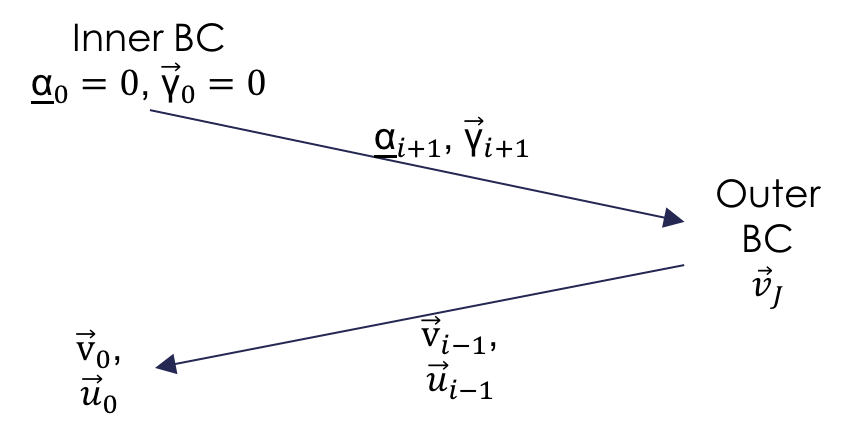
\includegraphics[width = 0.5 \textwidth]{Overview.png}
\caption{A diagrammatic overview of the Henyey method, showing what is being evaluated at each stage of the code.  The arrows represent the two recurrence relations, with the inwards arrow progressively calculating the solution as it works back towards the centre of the grid.}
\end{center}
\end{figure}


This code was built from scratch, and tested extensively in various situations, particularly assessing the differences between analytically equivalent expressions of the recurrence relations and the differences between different applications of the boundary conditions.  The numerical components were also extensively tested, including ensuring the accuracy of matrix inversion, particularly in the case of small determinants; a structure to deal with the manipulation of complex matrices was included and tested; and ...







\section{Implementing the equations}

This section discusses the more 














\section{Acknowledgements}

I would like to acknowledge MESA, \cite{Paxton2011}. http://mesa.sourceforge.net/index.html

This research has made use of the NASA Exoplanet Archive, which is operated by the California Institute of Technology, under contract with the National Aeronautics and Space Administration under the Exoplanet Exploration Program.





\bibliographystyle{plain}
\bibliography{library}









\newpage

\appendix

\section{Stellar Oscillation Equations} \label{ap:Osc}




\end{document}  
